\documentclass[conference]{IEEEtran}
\usepackage{graphicx}
\IEEEoverridecommandlockouts
% The preceding line is only needed to identify funding in the first footnote. If that is unneeded, please comment it out.
\usepackage{cite}
\usepackage{amsmath,amssymb,amsfonts}
\usepackage{algorithmic}
\usepackage{graphicx}
\usepackage{textcomp}
\usepackage{xcolor}
\def\BibTeX{{\rm B\kern-.05em{\sc i\kern-.025em b}\kern-.08em
    T\kern-.1667em\lower.7ex\hbox{E}\kern-.125emX}}
\begin{document}

\title{BareTag Tool-Tracker\\
{\footnotesize {Team 3 - University of Massachusetts Amherst Senior Design Project 2025 }}
}

\author{
    \IEEEauthorblockN{Sean Brown}
    \IEEEauthorblockA{\textit{Computer Engineering} \\
    \textit{Logistics Lead}\\}
    \and
    \IEEEauthorblockN{Connor McGarry}
    \IEEEauthorblockA{\textit{Computer Engineering} \\
    \textit{Hardware Lead}\\}
    \and
    \IEEEauthorblockN{Ken Su}
    \IEEEauthorblockA{\textit{Computer Engineering} \\
    \textit{Budget Lead}\\}
    \and
    \IEEEauthorblockN{Walter Tebbetts}
    \IEEEauthorblockA{\textit{Computer Engineering} \\
    \textit{Software Lead}\\}
    \and
    \IEEEauthorblockN{Professor Jeremy Gummeson}
    \IEEEauthorblockA{\textit{UMass Amherst ECE Faculty} \\
    \textit{Advisor}\\}
}

\maketitle

\begin{abstract}
    Over the past 10 years, the majority of tools on a construction 
    site have converted from wired to battery-powered. While this 
    makes tools easy to move around, it also makes them easy to misplace
    and an easier target for theives. Data indicates that the construction
    idustry suffered nearly \$1,000,000,000 in loses due to tool theft in
    2023 alone [1], strongly indicating the need for a robust and effective 
    theft mitigation system. We propose the BareTag Tool-Tracker, a novel
    approach to tool tracking that utilizes Ultra-Wideband(UWB) and Bluetooth 
    Low-Energy(BLE) radio in order to real-time track tools, materials, or other 
    valuable items on a construction site. The system utilizes a series
    of pre-placed Anchor posts, that send UWB pings to a Tag that is connected
    to a tool. Each Anchor can then calculate its distance to a Tag, relaying
    that information to a Base station over Long Range(LoRa) radio. The 
    base station runs the aggregated distance data through a multilateration
    algorithm that can calculate the Tag's location with $\pm$ 10 cm accuracy.
    The calculated location is then output to a local terminal, as well as 
    uploaded to a cloud database for future reference. Altogether, the BareTag Tool-Tracker
    is highly accurate ($\pm$ 10 cm), low-power (1 year of battery life), and
    scalable (increase range by adding additional Anchors).
\end{abstract}

\begin{IEEEkeywords}
component, formatting, style, styling, insert
\end{IEEEkeywords}

\section{Introduction}
On constructions sites tools are constantly being misplaced or passed around causing workers to spend extra time searching and waiting before returning to their assignments. Furthermore, in recent years research has shown that theft on constructions sites has built up costs for construction companies and slowing down projects, very detrimental for small companies. In recent years many different approaches have been taken to solve this growing issue. 
\subsection{Significance}
In 2016 it was estimated that in the United States alone \$1,000,000,000 worth of construction tools were stolen [1]. A survey by the Charted Institute of Building discovered that out of the 1000 construction mangers interviewed, a third responded that they had experienced theft weekly on their sites. It was estimated that each of these weekly incidents cost the business an average of \$6,000, in some cases, in a single night the site had lost \$100,000 worth of equipment [2]. What’s worse is that this is a growing case. The FBI has reported that in 2021, theft on construction sites had outgrown theft in convenience stores [3]. Many managers have reported that these incidents have escalated to organized crime with evidence of sophisticated planning and coordinated executions. [2]. Theft on the site is not only costly to the business owners but also even more inconvenient for the construction workers and their managers. Due to the lack of proper tools construction workers may not continue with their assignments and managers have to keep pushing deadlines. The result of this costs the business not just in extra wages, but also extra insurance and the company’s reputation [2]. 

\section{DESIGN}

This section describes the system design including design alternatives, design justifications, and hardware and software block diagrams.

\section{Overview}
At a high level, the BareTag Tool Tracker utilizes Ultra-Wideband (UWB), Bluetooth Low Energy (BLE), and LoRa radio in order to real-time track an item's location on a construction site. The technology at the core of our design is UWB radio. UWB radio is a form of radio communication that utilizes pulses of radio energy at specifically timed intervals in order to transmit information. This protocol is not ideal for data communication, but is very accurate in performing distance ranging. With two UWB transceivers, one configured as the controller (Anchor) and the other configured as the responder (Tag), the controller can send a UWB ping to the responder. The responder will almost immediately send back a response ping, the controller can then use the time between when it sent its ping to when it received the response ping, in order to calculate the distance between the two transceivers. 

\begin{figure}
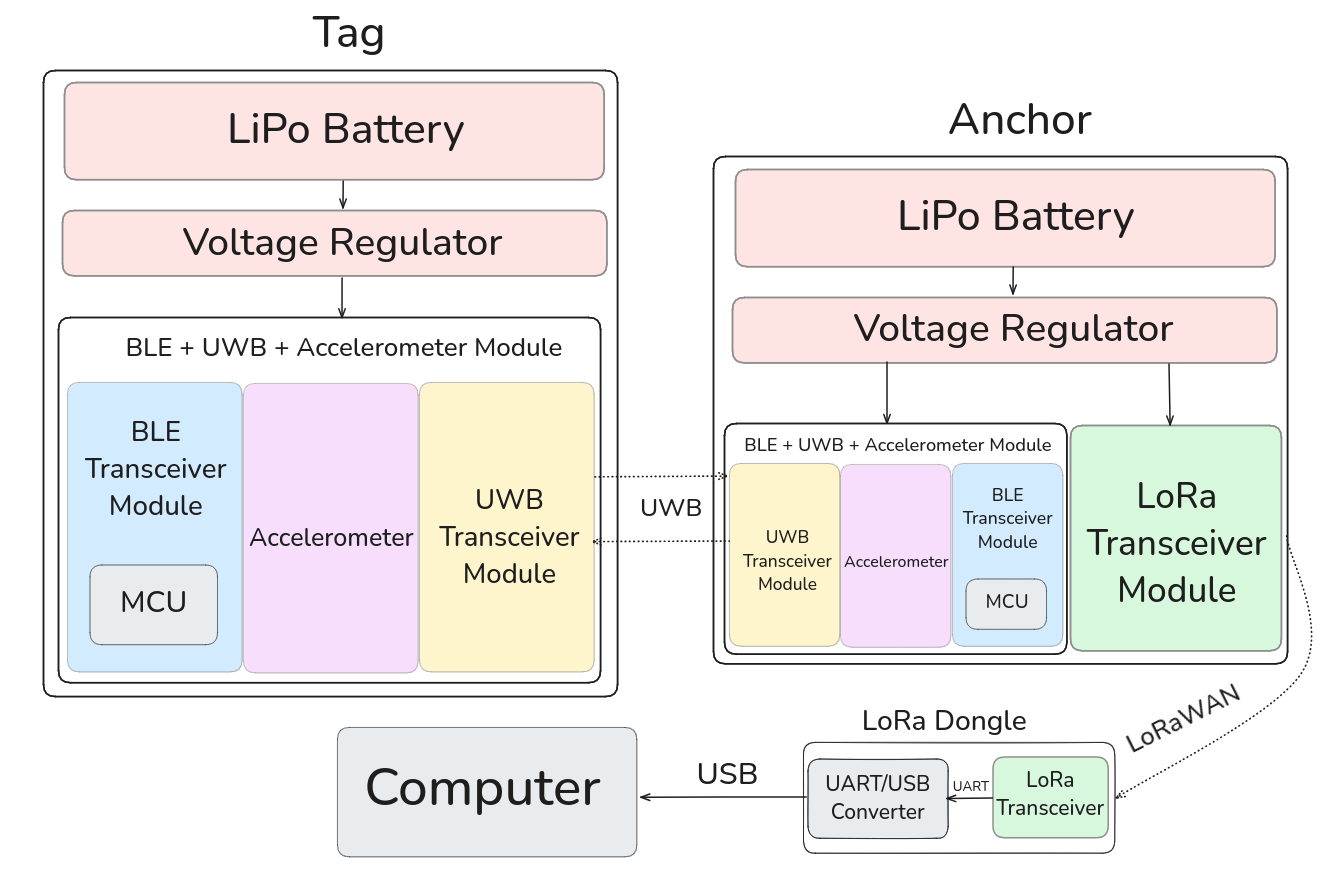
\includegraphics[scale=0.185]{Screenshot from 2024-10-18 21-37-02.png}
\caption{Full system hardware block diagram}
\end{figure}

\subsection{Tag}\label{AA}
The Tag refers to the trackable device that will be attached to the tools on a worksite. The goal is for the Tags to be less than 31.9mm2, which is of a similar size to the Apple Airtag. The thickness of the Tags is aimed to be under 16mm, with the primary contributor to this size being the pouch cell 290mAh Lithium Polymer battery. The peak current draw of the Tag is 45mA and is out of the range that a coin cell could support, which led to the decision to use a LiPo that fits within our area size goals at 25 mm x 28mm. We are aiming for a one year battery life.
The primary part of the Tag is the Qorvo DWM3001C. This module is driven by the nRF52833 MCU, and includes BLE, UWB, and accelerometer functionality. The DWM3001 provides UWB functionality and has an integrated PCB antenna which requires a keep-out zone in the Tag. BLE is provided by the nRF52833. This MCU is built on an ARM Cortex M4 and operates in the 2.4GHz band. This MCU is programmable over JTAG and thus requires a JTAG interface to be added to the Tag PCBs. The accelerometer is the LIS12DH, and is used to wake up the module upon motion detection. The module will set the interrupt pin on the DWM3001 high when there is motion detected. Otherwise, the Tag is in a low power mode to save battery life and is not receiving UWB pings. Therefore, before the tag goes to sleep the location needs to be checked to determine the resting location. The Tag has the BLE radio turned off until it exits the UWB perimeter, at which point an interrupt pin turns it on to integrate into the Apple Find My network. At this point, the UWB module turns off to conserve power. The accelerometer still regulates the power mode of the Tag depending on motion to conserve power. This device draws a lot of concepts from ECE 523 and ECE 304, both of which have a heavy focus on minimizing power consumption via software and component selection.
The TPS79933 voltage regulator has an output of 3.3V when the input voltage is over 3.475V. This component is used in both the Tags and Anchors as both devices operate on a 3.7V input battery with 3.3V ideal operating voltage. 


\subsection{Anchor}
There needs to exist at least 3 anchors for the coordinates to be transmitted to the user. This is performed through multilateration. The Anchors use the same Qorvo DWM3001C modules as on the Tags as all of the submodules have a use case here too. The Anchors use UWB to ping the Tag and determine its location within the area defined by the proximity of the other anchors. They operate on this data using the nRF52833 MCU and send it to a host device over LoRaWAN. The RYLR998 LoRa module in the Anchors operates within the required range for LoRaWAN of 902.3 to 914.9 MHz. This module communicates with the MCU via UART. The use of these LoRa modules means that the Host Device does not need to be exactly on the site of the construction due to the kilometers of range that LoRa supports. We will build the LoRaWAN protocol on top of LoRa using the nRF52833 MCU. The use of this MCU also means that we can take advantage of the BLE it provides and use it for a variety of functions. The GPS coordinates of the Anchors must be known in order to get the real-world position of the Tags. We can also use BLE to communicate with an anchor to alert that a Tag that is in BLE mode has been returned to the UWB-supported area. These features result in  more power consumption than the Tags, so a 2.2Ah Lithium Ion battery is used. This is possible due to less size constraints for the Anchors than of the Tag. The size of the Anchor is not a specification that matters, however they will be able to be mounted on posts or stuck in different site locations depending on the desired use and area to cover.
As stated before, the TPS79933 voltage regulator outputs 3.3V, which is the ideal operating voltage for the DWM3001C, along with the LoRa module. 


\subsection{Lora Dongle}
This device is a RYLR998 operating over a USB - UART connection with the Host Device. It allows for the Host Device to receive the Tag coordinate data and operate on it. The size of this device should account for the LoRa module plus a USB/UART converter (CP2102N). The size should be similar to that of a USB hub, as to not be an inconvenience to have attached to a small host device. As such, the dimensions should be approximately 32 x 18 x 8 mm based on a combination of the component dimensions. 
The Dongle receives power from the CP2102N over a wired USB-C connection, so there is no need for an external power supply. 


\subsection{Host Device}

This device can be whatever system a supervisor desires to use as long as it can support a physical USB/Serial connection, or do so using adapters. The Host Device is backhauling the location data of each Tag to a database where the history of the tag locations can be mapped out to determine the daily path. This information is also displayed in real time on a map of the desired area. The Host Device is also running the macless-haystack Find My server, which acts as a means for tracking the Tags that have left the UWB area and are now using BLE to integrate with the Apple Find My network. The tags all have unique IDs that can be linked to tools or equipment, making it easy to parse the data and determine what items have been in what location. 

\subsection{Some Common Mistakes}\label{SCM}
\begin{itemize}
\item The word ``data'' is plural, not singular.
\item The subscript for the permeability of vacuum $\mu_{0}$, and other common scientific constants, is zero with subscript formatting, not a lowercase letter ``o''.
\item In American English, commas, semicolons, periods, question and exclamation marks are located within quotation marks only when a complete thought or name is cited, such as a title or full quotation. When quotation marks are used, instead of a bold or italic typeface, to highlight a word or phrase, punctuation should appear outside of the quotation marks. A parenthetical phrase or statement at the end of a sentence is punctuated outside of the closing parenthesis (like this). (A parenthetical sentence is punctuated within the parentheses.)
\item A graph within a graph is an ``inset'', not an ``insert''. The word alternatively is preferred to the word ``alternately'' (unless you really mean something that alternates).
\item Do not use the word ``essentially'' to mean ``approximately'' or ``effectively''.
\item In your paper title, if the words ``that uses'' can accurately replace the word ``using'', capitalize the ``u''; if not, keep using lower-cased.
\item Be aware of the different meanings of the homophones ``affect'' and ``effect'', ``complement'' and ``compliment'', ``discreet'' and ``discrete'', ``principal'' and ``principle''.
\item Do not confuse ``imply'' and ``infer''.
\item The prefix ``non'' is not a word; it should be joined to the word it modifies, usually without a hyphen.
\item There is no period after the ``et'' in the Latin abbreviation ``et al.''.
\item The abbreviation ``i.e.'' means ``that is'', and the abbreviation ``e.g.'' means ``for example''.
\end{itemize}
An excellent style manual for science writers is \cite{b7}.

\subsection{Authors and Affiliations}
\textbf{The class file is designed for, but not limited to, six authors.} A 
minimum of one author is required for all conference articles. Author names 
should be listed starting from left to right and then moving down to the 
next line. This is the author sequence that will be used in future citations 
and by indexing services. Names should not be listed in columns nor group by 
affiliation. Please keep your affiliations as succinct as possible (for 
example, do not differentiate among departments of the same organization).

\subsection{Identify the Headings}
Headings, or heads, are organizational devices that guide the reader through 
your paper. There are two types: component heads and text heads.

Component heads identify the different components of your paper and are not 
topically subordinate to each other. Examples include Acknowledgments and 
References and, for these, the correct style to use is ``Heading 5''. Use 
``figure caption'' for your Figure captions, and ``table head'' for your 
table title. Run-in heads, such as ``Abstract'', will require you to apply a 
style (in this case, italic) in addition to the style provided by the drop 
down menu to differentiate the head from the text.

Text heads organize the topics on a relational, hierarchical basis. For 
example, the paper title is the primary text head because all subsequent 
material relates and elaborates on this one topic. If there are two or more 
sub-topics, the next level head (uppercase Roman numerals) should be used 
and, conversely, if there are not at least two sub-topics, then no subheads 
should be introduced.

\subsection{Figures and Tables}
\paragraph{Positioning Figures and Tables} Place figures and tables at the top and 
bottom of columns. Avoid placing them in the middle of columns. Large 
figures and tables may span across both columns. Figure captions should be 
below the figures; table heads should appear above the tables. Insert 
figures and tables after they are cited in the text. Use the abbreviation 
``Fig.~\ref{fig}'', even at the beginning of a sentence.

\begin{table}[htbp]
\caption{Table Type Styles}
\begin{center}
\begin{tabular}{|c|c|c|c|}
\hline
\textbf{Table}&\multicolumn{3}{|c|}{\textbf{Table Column Head}} \\
\cline{2-4} 
\textbf{Head} & \textbf{\textit{Table column subhead}}& \textbf{\textit{Subhead}}& \textbf{\textit{Subhead}} \\
\hline
copy& More table copy$^{\mathrm{a}}$& &  \\
\hline
\multicolumn{4}{l}{$^{\mathrm{a}}$Sample of a Table footnote.}
\end{tabular}
\label{tab1}
\end{center}
\end{table}

\begin{figure}[htbp]
\caption{Example of a figure caption.}
\label{fig}
\end{figure}

Figure Labels: Use 8 point Times New Roman for Figure labels. Use words 
rather than symbols or abbreviations when writing Figure axis labels to 
avoid confusing the reader. As an example, write the quantity 
``Magnetization'', or ``Magnetization, M'', not just ``M''. If including 
units in the label, present them within parentheses. Do not label axes only 
with units. In the example, write ``Magnetization (A/m)'' or ``Magnetization 
\{A[m(1)]\}'', not just ``A/m''. Do not label axes with a ratio of 
quantities and units. For example, write ``Temperature (K)'', not 
``Temperature/K''.

\section*{Acknowledgment}

The preferred spelling of the word ``acknowledgment'' in America is without 
an ``e'' after the ``g''. Avoid the stilted expression ``one of us (R. B. 
G.) thanks $\ldots$''. Instead, try ``R. B. G. thanks$\ldots$''. Put sponsor 
acknowledgments in the unnumbered footnote on the first page.

\section*{References}

Please number citations consecutively within brackets \cite{b1}. The 
sentence punctuation follows the bracket \cite{b2}. Refer simply to the reference 
number, as in \cite{b3}---do not use ``Ref. \cite{b3}'' or ``reference \cite{b3}'' except at 
the beginning of a sentence: ``Reference \cite{b3} was the first $\ldots$''

Number footnotes separately in superscripts. Place the actual footnote at 
the bottom of the column in which it was cited. Do not put footnotes in the 
abstract or reference list. Use letters for table footnotes.

Unless there are six authors or more give all authors' names; do not use 
``et al.''. Papers that have not been published, even if they have been 
submitted for publication, should be cited as ``unpublished'' \cite{b4}. Papers 
that have been accepted for publication should be cited as ``in press'' \cite{b5}. 
Capitalize only the first word in a paper title, except for proper nouns and 
element symbols.

For papers published in translation journals, please give the English 
citation first, followed by the original foreign-language citation \cite{b6}.

\begin{thebibliography}{00}
\bibitem{b1} G. Eason, B. Noble, and I. N. Sneddon, ``On certain integrals of Lipschitz-Hankel type involving products of Bessel functions,'' Phil. Trans. Roy. Soc. London, vol. A247, pp. 529--551, April 1955.
\bibitem{b2} J. Clerk Maxwell, A Treatise on Electricity and Magnetism, 3rd ed., vol. 2. Oxford: Clarendon, 1892, pp.68--73.
\bibitem{b3} I. S. Jacobs and C. P. Bean, ``Fine particles, thin films and exchange anisotropy,'' in Magnetism, vol. III, G. T. Rado and H. Suhl, Eds. New York: Academic, 1963, pp. 271--350.
\bibitem{b4} K. Elissa, ``Title of paper if known,'' unpublished.
\bibitem{b5} R. Nicole, ``Title of paper with only first word capitalized,'' J. Name Stand. Abbrev., in press.
\bibitem{b6} Y. Yorozu, M. Hirano, K. Oka, and Y. Tagawa, ``Electron spectroscopy studies on magneto-optical media and plastic substrate interface,'' IEEE Transl. J. Magn. Japan, vol. 2, pp. 740--741, August 1987 [Digests 9th Annual Conf. Magnetics Japan, p. 301, 1982].
\bibitem{b7} M. Young, The Technical Writer's Handbook. Mill Valley, CA: University Science, 1989.
\end{thebibliography}
\vspace{12pt}
\color{red}
IEEE conference templates contain guidance text for composing and formatting conference papers. Please ensure that all template text is removed from your conference paper prior to submission to the conference. Failure to remove the template text from your paper may result in your paper not being published.

\end{document}
